\documentclass{article} % For LaTeX2e
\usepackage{nips15submit_e,times}
\usepackage{hyperref}
\usepackage{url}
%\documentstyle[nips14submit_09,times,art10]{article} % For LaTeX 2.09
\usepackage{amsmath}
\usepackage{graphicx}
\usepackage{listings}
\usepackage{subfigure}
\title{Handwritten Digits with Multilayer Backpropagation Neural Networks}


\author{
Shilin Zhu \\
Ph.D. student, Computer Science\\
UCSD\\
La Jolla, CA \\
\texttt{shz338@eng.ucsd.edu} \\
\And
Yunhui Guo\\
Ph.D. student, Computer Science\\
UCSD\\
La Jolla, CA \\
\texttt{yug185@eng.ucsd.edu} \\
}

% The \author macro works with any number of authors. There are two commands
% used to separate the names and addresses of multiple authors: \And and \AND.
%
% Using \And between authors leaves it to \LaTeX{} to determine where to break
% the lines. Using \AND forces a linebreak at that point. So, if \LaTeX{}
% puts 3 of 4 authors names on the first line, and the last on the second
% line, try using \AND instead of \And before the third author name.

\newcommand{\fix}{\marginpar{FIX}}
\newcommand{\new}{\marginpar{NEW}}

\nipsfinalcopy % Uncomment for camera-ready version

\begin{document}
\maketitle
\section{Abstract}

\section{Classification}
\subsection{Mini-batch gradient descent}
In this section, we use mini-batch gradient descent to classify the MNIST dataset. We split the 60000 images in the training set into two parts: the first 50000 images are used to train the model, the last 10000 images are used as validation set to do early stopping. We stop the training procedure once the loss on the validation set goes up and we save the weights that achieves the minimum loss on the validation set. And there are 10000 images in the test set.

We use one hidden layer of 64 nodes, and the mini-batch size is 128. We use a learning rate of 0.01 and sigmoid activation function. We use standard normal distribution to initialize the weights and biases. For the weights, we multiply 0.01 to prevent large initialized values. We run the network for 60 epoches.

 We report the accuracy and loss on the training set, test se and validation set every batch. The following graphs show the accuracy and loss over each batch on different sets. Without any tricks, after 60 epoches, the accuracy on the test set is 0.9308\%. This is no early stopping occurs, the possible reason is that the choice of learning is small

\begin{figure*} [!htbp]
	\subfigure[]{   
		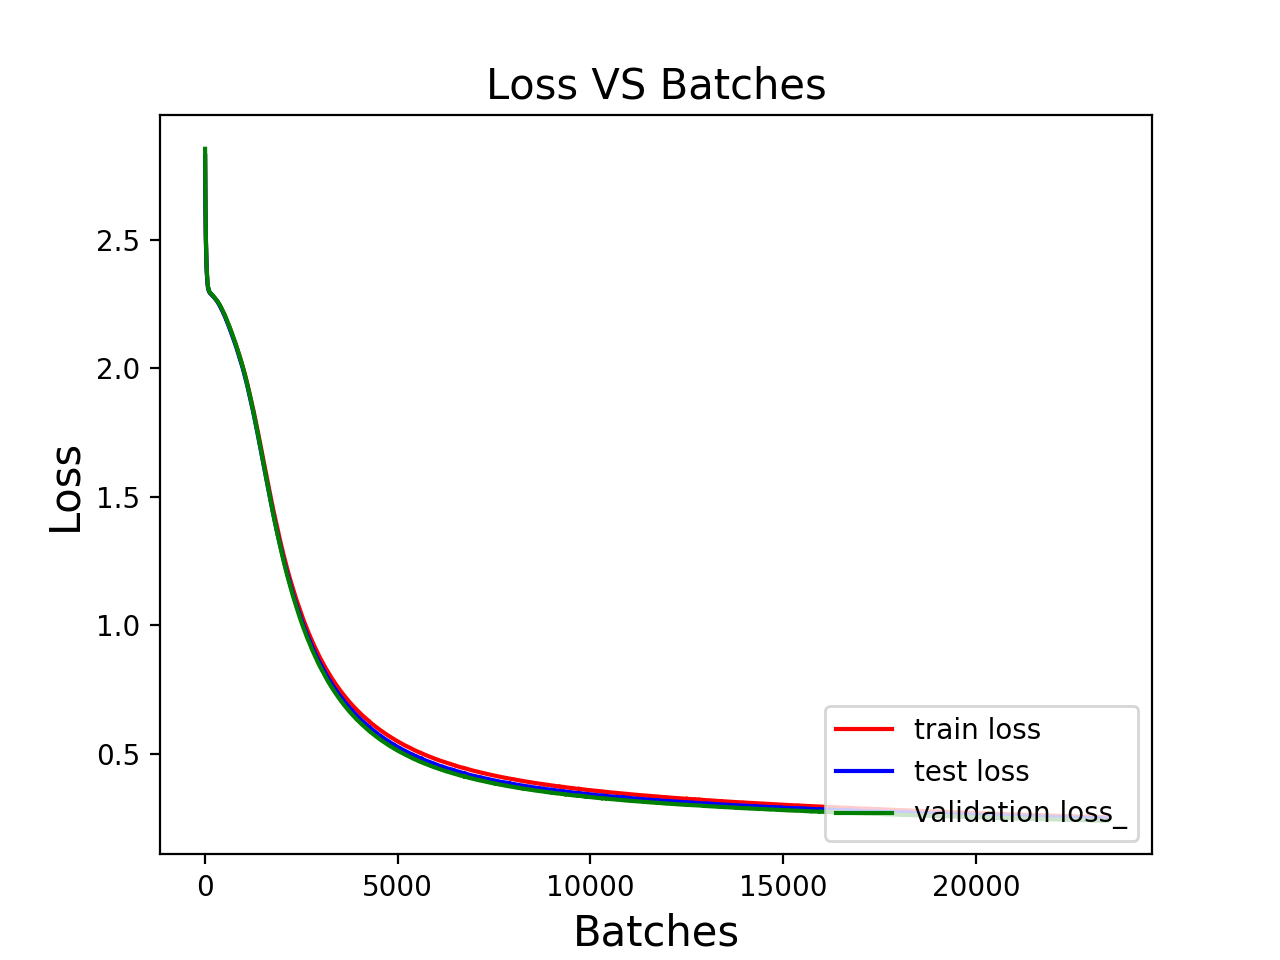
\includegraphics[width=3in]{images/3e_loss_64_hidden.png}}
	\subfigure[]{   
		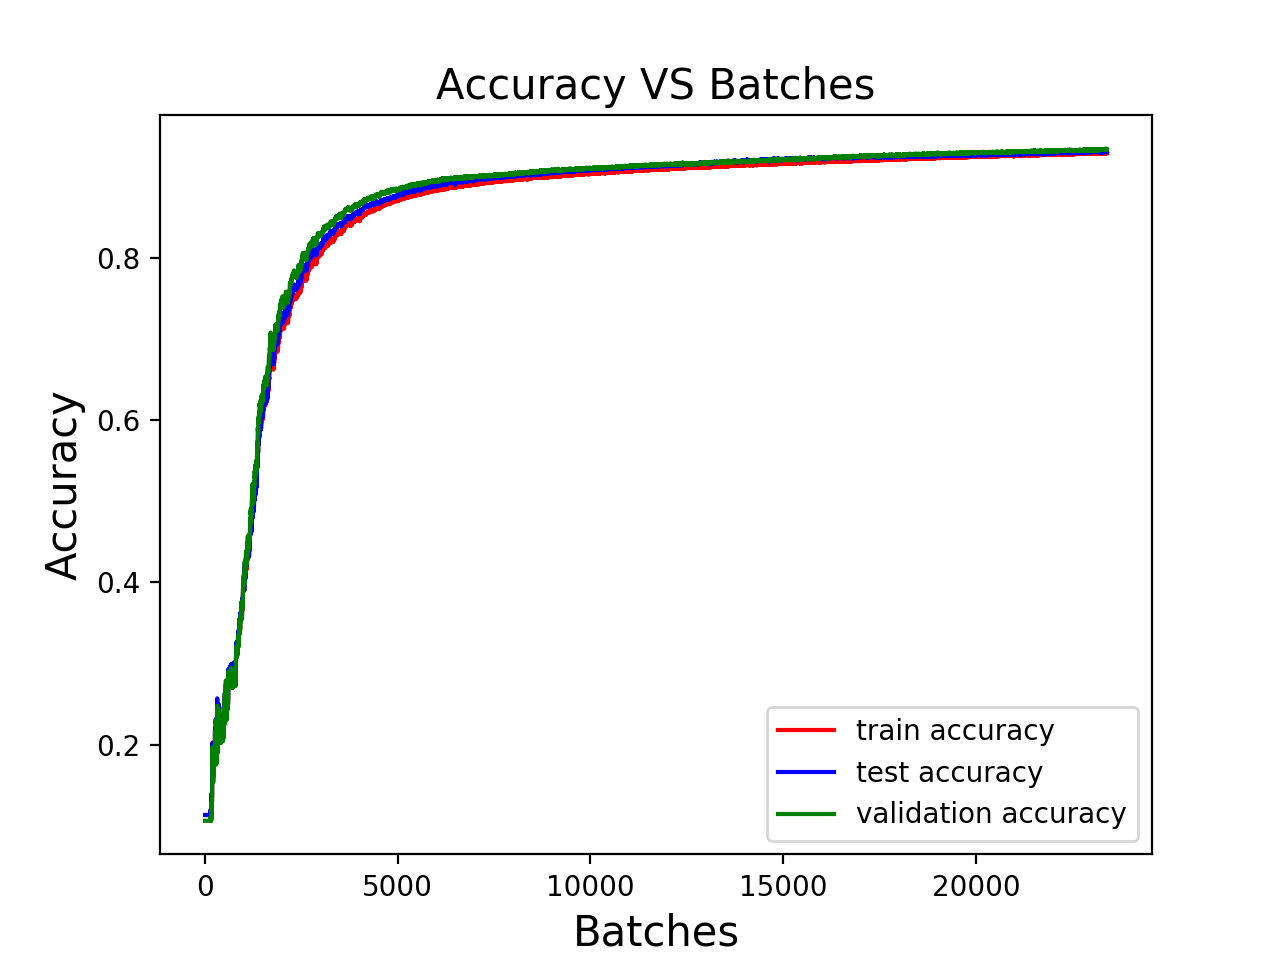
\includegraphics[width=3in]{images/3e_accuracy_64_hidden.png}}
	
	\caption{The loss and accuacy of different sets over the batches. }  
	
\end{figure*}

\section{Adding the “Tricks of the Trade"}


\section{Experiment with Network Topology}

\subsection{Experiments with differnet hidden units}
We use a momentum of 0.9 and use the sigmoid in Section 4.4 of ``lecun98efficient.pdf". The initialization method of weights are as described in 4 (c) in Programming assignment 2. Learning rate is 0.01.

First, we half the hidden units. Now we have a network of 3 layers with a hidden layer with 32 nodes. We run the network for 60 epoches except early stopping occurs.

\subsection{Doubling the hidden layers}

\subsection{More tricks}
In this section, in order to improve the preformance of the network, we consider the following tricks. In our experiments, we found that the network can achieve fast convergence and higher test accuracy with the tricks.

\subsubsection{ReLU}
We consider using ReLU as the activation function. The ReLU function can be 

\[
\textnormal{ReLU}(x) =\left\{
\begin{array}{ll}
x \qquad \textnormal{if x $>$ 0,}\\
0 \qquad \textnormal{otherwise,}
\end{array}
\right.
\]

The gradient of ReLU can be caculated as,
 \[
\textnormal{dReLU}(x) =\left\{
\begin{array}{ll}
1 \qquad \textnormal{if x $>$ 0,}\\
0 \qquad \textnormal{otherwise,}
\end{array}
\right.
\]



The following graphs shows the 


\subsubsection{Leaky ReLU}

We consider using leaky ReLU as the activation function. The leaky ReLU function can be 

\[
\textnormal{LeakyReLU}(x) =\left\{
\begin{array}{ll}
x \qquad \textnormal{if x $>$ 0,}\\
0.01x \qquad \textnormal{otherwise,}
\end{array}
\right.
\]

The gradient of leaky ReLU can be caculated as,
\[
\textnormal{dLeakyReLU}(x) =\left\{
\begin{array}{ll}
1 \qquad \textnormal{if x $>$ 0,}\\
0.01 \qquad \textnormal{otherwise,}
\end{array}
\right.
\]
\subsubsection{Nesterov momentum}
We consider using Nesterov momentum.

\subsubsection{Xavier initializtion}
We consider using Xavier initializtion to initialize the weights.


\subsubsection{Dropout}


\end{document}
